\subsection{Qualitative Auswertung}

\todo[noline]{Zahlenformat überprüfen}

Im Rahmen der Testsitzungen wurden 20 verschiedene Usability-Probleme identifiziert. Diese wurden entweder im Zuge von \ac{CTA} von den Teilnehmer:innen bemängelt, oder durch Verwirrung, Zögern und fehlerhafte Nutzung festgestellt.

\begin{figure}[!ht]
  \colorlet{presentation}{plot1}
  \colorlet{interaction}{plot2}
  \colorlet{content}{plot3}
  \colorlet{technical}{plot4}
  \centering
  \begin{tikzpicture}
    \begin{axis}[
        xbar=0pt,
        xmajorgrids=true,
        xtick={0,...,10},
        xmin=0,
        xmax=6,
        xlabel={Absolute Häufigkeit},
        /pgf/bar shift=0pt,
        legend style={legend cell align=left},
        legend pos=south east,
        axis y line*=none,
        axis x line*=bottom,
        tick label style={font=\footnotesize},
        legend style={font=\footnotesize},
        label style={font=\footnotesize},
        width=.6\textwidth,
        bar width=3.5mm,
        ymin=1,
        ytick={1,...,20},
        ytick style={draw=none},
        yticklabels={
            {\hyperref[p:functionlist]{Übersichtlichkeit Funktionsliste (T)}},
            {\hyperref[p:präfix]{Präfix von Objektklassen (S)}},
            {\hyperref[p:functions]{Details zu Funktionen (R)}},
            {\hyperref[p:queryables]{Benennung Abfragbare Felder (Q)}},
            {\hyperref[p:meta]{Metadaten von Szenario-Feldern (P)}},
            {\hyperref[p:filter]{Automatische Typfilterung (O)}},
            {\hyperref[p:overload]{Auswahl von Überladungen (N)}},
            {\hyperref[p:scroll]{Probleme mit Scrollen (M)}},
            {\hyperref[p:quelle]{Zugriff auf die Quelldaten (L)}},
            {\hyperref[p:statisch]{Angabe von statischen Werten (K)}},
            {\hyperref[p:mitte]{Benennung mittlerer Bereich (J)}},
            {\hyperref[p:speichern]{Benennung des Speichern-Buttons (I)}},
            {\hyperref[p:drag]{Drag \& Drop (H)}},
            {\hyperref[p:ersetzen]{Ersetzen von Einträgen (G)}},
            {\hyperref[p:datentyp]{Datentyp von Szenario-Feldern (F)}},
            {\hyperref[p:parameterübernahme]{Parameterübernahme bei Überladungen (E)}},
            {\hyperref[p:parameter]{Details zu Parametern (D)}},
            {\hyperref[p:icons]{Icons für Datentypen (C)}},
            {\hyperref[p:attribute]{Anzeige von Attributen in Ziel (B)}},
            {\hyperref[p:bedienreihenfolge]{Bedienreihenfolge von Funktionen (A)}},
          },
        area legend,
        y=6mm,
        enlarge y limits={abs=0.625},
        every axis plot/.append style={fill}
      ]
      \addplot[interaction]  coordinates {(0,0)};  \addlegendentry{Interaktion (8)}
      \addplot[presentation] coordinates {(0,0)};  \addlegendentry{Darstellung (7)}
      \addplot[content]      coordinates {(0,0)};  \addlegendentry{Inhalt (4)}
      \addplot[technical]    coordinates {(0,0)};  \addlegendentry{Technisch (1)}

      \addplot[presentation] coordinates {(1,1)};  % Übersichtlichkeit Funktionsliste
      \addplot[content]      coordinates {(2,2)};  % Präfix von Objektklassen
      \addplot[content]      coordinates {(2,3)};  % Details zu Funktionen
      \addplot[presentation] coordinates {(2,4)};  % Benennung Abfragbare Felder
      \addplot[presentation] coordinates {(2,5)};  % Metadaten von Szenario-Feldern
      \addplot[interaction]  coordinates {(2,6)};  % automatische Typfilterung
      \addplot[interaction]  coordinates {(2,7)};  % Auswahl von Überladungen
      \addplot[technical]    coordinates {(3,8)};  % Probleme mit Scrollen
      \addplot[content]      coordinates {(3,9)};  % Zugriff auf die Quelldaten
      \addplot[interaction]  coordinates {(3,10)}; % Angabe von statischen Werten
      \addplot[presentation] coordinates {(4,11)}; % Benennung mittlerer Bereich
      \addplot[presentation] coordinates {(4,12)}; % Benennung des Speichern-Buttons
      \addplot[interaction]  coordinates {(4,13)}; % Drag \& Drop
      \addplot[interaction]  coordinates {(4,14)}; % Ersetzen von Einträgen
      \addplot[interaction]  coordinates {(4,15)}; % Datentyp von Szenario-Feldern
      \addplot[interaction]  coordinates {(4,16)}; % Parameterübernahme bei Überladungen
      \addplot[content]      coordinates {(5,17)}; % Details zu Parametern
      \addplot[presentation] coordinates {(5,18)}; % Icons für Datentypen
      \addplot[presentation] coordinates {(5,19)}; % Anzeige von Attributen in Ziel
      \addplot[interaction]  coordinates {(6,20)}; % Bedienreihenfolge von Funktionen
    \end{axis}
  \end{tikzpicture}
  \caption{Häufigkeit des Auftretens verschiedener Probleme während der Usability-Studie. Gezählt wird die Anzahl der Testsitzungen, in der das jeweilige Problem aufgetaucht ist.}
  \label{figure:problems}
\end{figure}

Abbildung \ref{figure:problems} listet die aufgetretenen Probleme, zusammen mit ihrer Häufigkeit auf. Hierbei wird die Anzahl der Testsitzungen gezählt, in denen das jeweilige Problem aufgetaucht ist. Es wird nicht zwischen der Stärke des Auftretens unterschieden: Von einer Testperson könnte nur ein Verbesserungsvorschlag geäußert worden sein, während eine andere Person durch das Problem eine Aufgabe nicht richtig absolvieren konnte. Außerdem wird der Härtegrad des Problems nicht bewertet. Eine Problem welches häufig auftritt könnte die Nutzer:innen zu einem geringeren Grad beeinträchtigt haben, während weniger häufig auftretende Probleme ein größeres Hindernis darstellen können. Diesbezüglich können sich auch die Meinungen der Teilnehmer:innen unterscheiden.

Die aufgetretenen Probleme können in vier Kategorien unterteilt werden. Diese sind in Abbildung \ref{figure:problems} farblich dargestellt. Außerdem wurde jedem Problem ein Buchstabe zugeordnet (A-T), über welchen zur zugehörigen Textstelle navigiert werden kann. Im Folgenden werden die Probleme, sortiert nach ihrer Kategorie, erläutert.

\subsubsection{Interaktionsprobleme}

Probleme dieser Art sind dadurch charakterisiert, das sie Hürden beim Bedienen der Oberfläche darstellen. Die Nutzer:innen erwarteten beispielsweise eine unterschiedliche Art der Benutzung, oder hatten Schwierigkeiten bestimmte Aktionen auszuführen. Insgesamt wurden 8 Interaktionsprobleme festgestellt.

\plabel{p:bedienreihenfolge}
Am Häufigsten wurde die Bedienreihenfolge von Funktionen \textbf{(A)} kritisiert. Der Block-Editor ist so konzipiert, dass zuerst die gewünschte Funktion gewählt, in das Zielfeld eingefügt wird und dann die dazugehörigen Parameter ausgesucht werden. In 6 Testsitzungen wurde dies thematisiert. Zu beachten ist, dass dieses Problem meistens im Zuge der Textverkettung im zweiten Szenario angesprochen wurde (Vgl. Anhang \ref{app:handout}). Ob dies daran liegt, dass es sich beim Großteil der Testsitzungen hierbei um den ersten Kontakt mit Funktionen handelt, oder dass die gleiche Aufgabe oft mithilfe von Operatoren in der Infixnotation gelöst wird, ist unklar. Vier Teilnehmer:innen äußerten sich nicht zur Art und Weise wie Funktionen im Editor eingesetzt werden und kamen ohne Probleme damit zurecht. Sie hatten alle Programmier- oder \ac{SQL}-Kenntnisse. Die restlichen 6 Personen konnten die Aufgabe zwar lösen, wählten zunächst jedoch andere Herangehensweisen oder merkten an, dass sie es gerne auch anders umgesetzt hätten. Drei von ihnen setzten zunächst den ersten Parameter ein, und wollten dann die Funktion darauf anwenden, während eine weitere Person im Nachhinein den Wunsch ausdrückte, dass es zusätzlich zu aktuellen Funktionsweise auch so gehen sollte. Eine von ihnen begründete diese Herangehensweise mit dem von ihr genutzten \ac{GIS}. Für sie war es nicht auf sofort ersichtlich, wie sie zwei Attribute miteinander verknüpfen kann. Zwei weitere Personen wollten im Rahmen der Textverkettung zunächst komplett auf Funktionen verzichten und die benötigten Attribute nacheinander in das Zielfeld klicken. Nachdem dies nicht möglich war, wollte eine von ihnen manuell die Schlüssel aus der Quelltabelle in das Zielfeld schreiben und mithilfe des Konkatenierungs-Operator (\texttt{||})\footnote{\url{https://www.postgresql.org/docs/9.1/functions-string.html}} verketten.

\plabel{p:parameterübernahme}
Beim Auswählen von Funktionsüberladungen werden die Parameter von einer Überladung nicht in die nächste übernommen \textbf{(E)}. Vier Personen waren davon verwirrt, dass die ersten, bereits ausgefüllten Parameter, leer sind, sobald eine Überladung mit mehr Parametern ausgewählt wird. Zwei von ihnen merkten an, dass die Anzahl der Parameter auch nach dem Ausfüllen anpassbar sein sollte, wobei eine von ihnen darauf einging dass es schwierig sein könnte, dies konsistent umzusetzen. Ein:e Teilnehmer:in erkannte, dass die zuvor eingetragenen Parameter in der Überladung mit weniger Parametern bestehen bleiben, und entfernte diese manuell, aus Angst dass dies Fehler verursachen könnte.

\plabel{p:datentyp}
\todo{Foto von Dropdown}
Der Datentyp von Feldern im Szenario-Modus \textbf{(F)} kann über ein Dropdown beim Button zum Hinzufügen von Feldern angepasst werden. Der Standardtyp ist Text. Im dritten Szenario werden Hausnummer abgefragt, welche als Ganzzahl vorliegen, es muss also ein passendes Feld erstellt werden. In 4 Testsitzungen kam es dadurch zu Verwirrungen, da die Teilnehmer:innen ein Textfeld ausgewählt hatten, und somit die Hausnummer nicht einfügen konnten. Das Dropdown zur Typauswahl wurde nicht sofort wahrgenommen, oder mit dieser Funktionalität verbunden. Eine Person bezeichnete das Dropdown zur Typauswahl als "unintuitiv" und schlug vor, die Anpassung des Typs erst nach Hinzufügen des Feldes durchzuführen. Eine weiterer Vorschlag bestand darin, Funktionen zum Konvertieren von Attributen bereitzustellen, oder dies automatisch durchzuführen. In Abbildung \ref{fig:type-dropdown} ist das beschriebene Dropdown zu sehen. Ein:e Teilnehmer:in wünschte sich, die im Rest der Anwendung genutzten Icons auch in diesem Menü wiederzufinden.

\begin{figure}
  \centering
  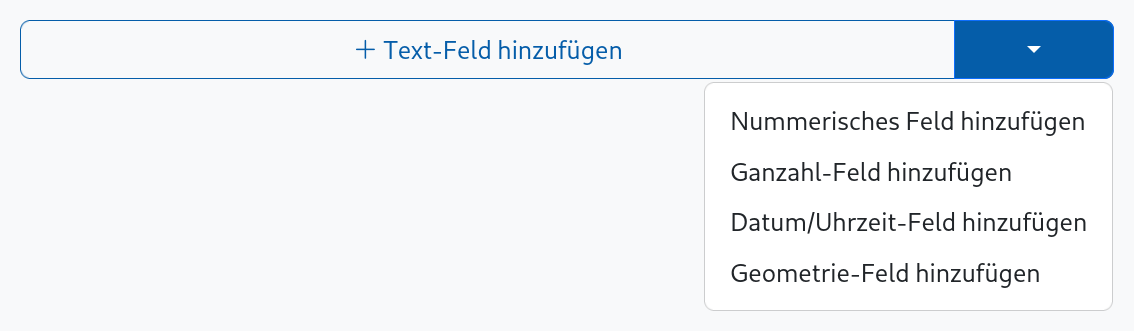
\includegraphics[width=.9\textwidth]{assets/datatype-dropdown.png}
  \caption{Dropdown zum Auswählen des Datentyps von Feldern im Szenario-Modus}
  \label{fig:type-dropdown}
\end{figure}

\plabel{p:ersetzen}
\plabel{p:drag}
\plabel{p:statisch}
\plabel{p:overload}
\plabel{p:filter}

\subsubsection{Darstellungsprobleme}

Auch die Darstellung von Informationen innerhalb des Block-Editors führte zu Problemen. Es wurden 8 Darstellungsprobleme identifiziert, welche von unklaren Bezeichnungen bis hin zu Icons reichen.

\plabel{p:attribute}
\plabel{p:icons}
\plabel{p:speichern}
\plabel{p:mitte}
\plabel{p:meta}
\plabel{p:queryables}
\plabel{p:functionlist}

\subsubsection{Inhaltliche Probleme}

\plabel{p:parameter}
\plabel{p:quelle}
\plabel{p:functions}
\plabel{p:präfix}

\subsubsection{Technische Probleme}

\plabel{p:scroll}
